\newif\ifalone
\alonefalse
\newif\iftalk
\talktrue

\ifalone
\documentclass{article}
\usepackage{graphicx}
\usepackage{natbib}
\usepackage{amsfonts}
\usepackage{amssymb}
\usepackage{amsthm}
\usepackage{bm}
\usepackage{Sweave}
\usepackage{lscape}
\usepackage{makeidx}
\usepackage{color}


\title{Continuous Random Interactions}

\author{Jarrod Hadfield (\texttt{j.hadfield@ed.ac.uk})}
\begin{document}
\maketitle
\else
\chapter{Continuous Random Interactions}
\label{chap4}
\fi


In Lecture \ref{chap3} we saw how we could define a linear model within a variance function and then interact these terms with a random effect. In the example, we did this in order to fit a \texttt{sex} by \texttt{dam} interaction:

\begin{Schunk}
\begin{Soutput}
us(sex):dam
\end{Soutput}
\end{Schunk}

The term entering into the variance function model was categorical, and we saw that by fitting the interaction we were essentially estimating the parameters of the covariance matrix:   

\begin{displaymath}
{\bf V}_{{\color{red} \texttt{dam}}}=
\left[
\begin{array}{ccc}
\sigma^{2}_{\color{blue}\texttt{Female}}&\sigma_{\color{blue}\texttt{Female}, \texttt{Male}}&\sigma_{\color{blue}\texttt{Female}, \texttt{UNK}}\\
\sigma_{\color{blue}\texttt{Female}, \texttt{Male}}&\sigma^{2}_{\color{blue}\texttt{Male}}&\sigma_{\color{blue}\texttt{Male}, \texttt{UNK}}\\
\sigma_{\color{blue}\texttt{Female}, \texttt{UNK}}&\sigma_{\color{blue}\texttt{Male}, \texttt{UNK}}&\sigma^{2}_{\color{blue}\texttt{UNK}}\\
\end{array}
\right]
\end{displaymath}

We are also free to define the variance function model with continuous covariates, or even a mixture of continuous and categorical factors, and the resulting covariance matrix is interpreted in the same way.

\section{Random Regression}

 As an example, we'll use a longitudinal data set on chicken growth (See Figure \ref{ChickWeight-fig}):

\begin{Schunk}
\begin{Sinput}
> data(ChickWeight)
\end{Sinput}
\end{Schunk}

The data consist of body weights (\texttt{weight}) for 50 chicks (\texttt{Chick}) measured up to 12 times over a 3 week period. The variable \texttt{Time} is the number of days since hatching, and \texttt{Diet} is a four level factor indicating the type of protein diet the chicks received.

\begin{Schunk}
\begin{Sinput}
> xyplot(weight ~ Time | Chick, data = ChickWeight)
\end{Sinput}
\end{Schunk}


\begin{figure}[!h]
\begin{center}
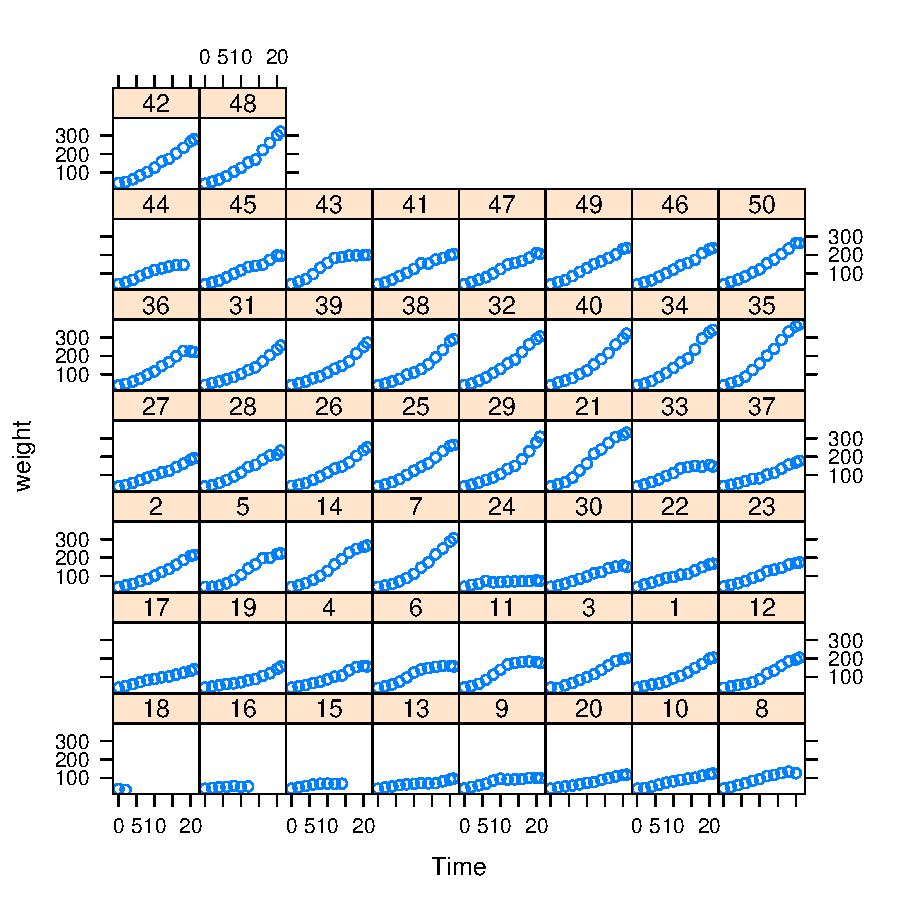
\includegraphics{Lecture4-005}
\end{center}
\caption{Weight data of 50 chicks from hatching until three weeks old.}
\label{ChickWeight-fig}
\end{figure}

Growth curves tend to be sigmoidal and so one of the non-linear growth curves such as the Gompertz or logistic may be a good starting model. However, these can be tricky to use and an alternative is to try and capture the form of the curve using polynomials. We'll start with a quadratic function at the population level and and fit chick as a random term:

\begin{Schunk}
\begin{Sinput}
> prior.m4a.1 <- list(R = list(V = 1e-16, n = -2), G = list(G1 = list(V = 1, 
+     n = 1)))
> m4a.1 <- MCMCglmm(weight ~ Diet + poly(Time, 2, raw = TRUE), 
+     random = ~Chick, data = ChickWeight, verbose = FALSE, pr = TRUE, 
+     prior = prior.m4a.1, saveX = TRUE, saveZ = TRUE)
\end{Sinput}
\end{Schunk}

We've saved the random chick effects so we can plot the predicted growth functions for each bird. For now we will just predict the growth function assuming that all birds were on Diet 1 (the intercept): 

\begin{Schunk}
\begin{Sinput}
> pop.int <- posterior.mode(m4a.1$Sol[, 1])
> pop.slope <- posterior.mode(m4a.1$Sol[, 5])
> pop.quad <- posterior.mode(m4a.1$Sol[, 6])
> chick.int <- posterior.mode(m4a.1$Sol[, c(7:56)])
\end{Sinput}
\end{Schunk}

We need to combine these parameter estimates with the polynomials for \texttt{Time} which are just the sequence $\texttt{Time}^{0}, \texttt{Time}^1, \texttt{Time}^2 \dots$ and so on. We can then plot the population expected population growth curve, and around that the predicted growth curves for each chick (we don't need to bother with $\texttt{Time}^{0}$ since this is always one):

\iftalk
\else

\begin{Schunk}
\begin{Sinput}
> pos.time <- seq(0, 21, length = 100)
> plot(pop.int + pop.slope * I(pos.time^1) + pop.quad * I(pos.time^2) ~ 
+     pos.time, type = "l", lwd = 2, ylim = c(-25, 400))
> for (i in 1:50) {
+     lines(pop.int + chick.int[i] + pop.slope * I(pos.time^1) + 
+         pop.quad * I(pos.time^2) ~ pos.time, col = "red", lty = 2)
+ }
\end{Sinput}
\end{Schunk}
\fi

\begin{figure}[!h]
\begin{center}
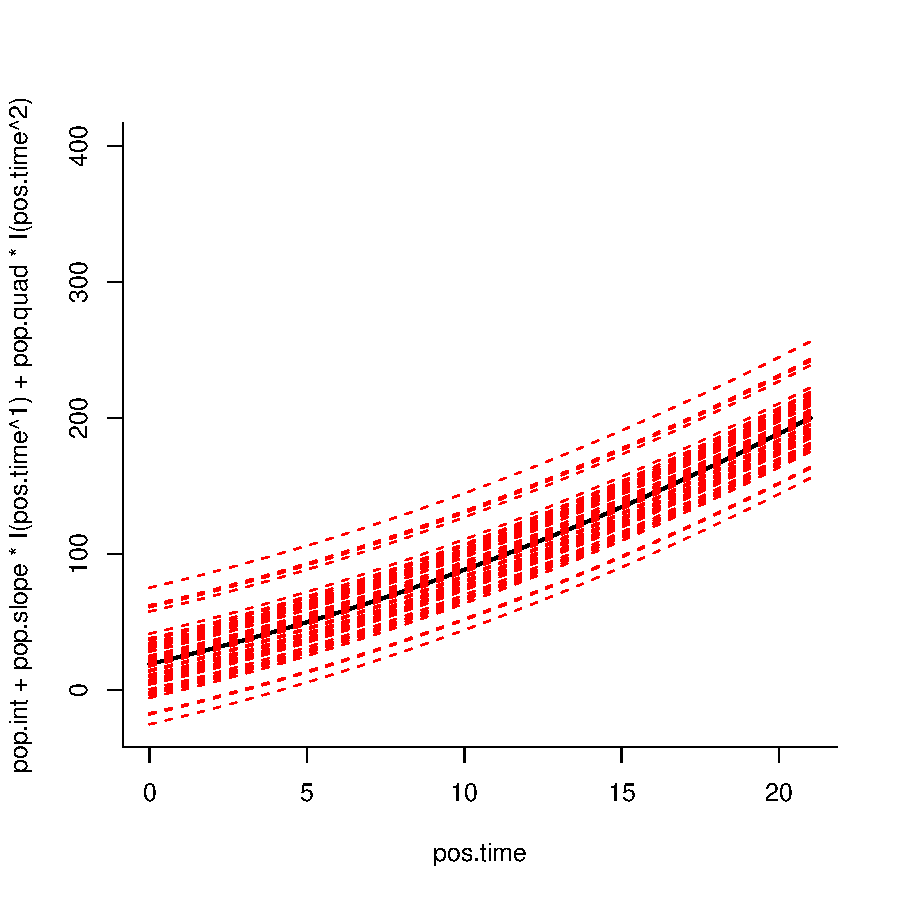
\includegraphics{Lecture4-011}
\end{center}
\caption{Predicted weights of each chick as a function of age. A quadratic population growth curve (black) is fitted with random chick intercepts.}
\label{CWpred.1-fig}
\end{figure}

The population growth curve is slightly convex because of the quadratic term, and the predictions for each chick are parallel to this curve. By fitting chick as a random effect we have allowed variation in the intercept only, and often this is not enough. We can get a feel for how well the model fits the data by overlaying the predictions with actual values. In the call to \texttt{MCMCglmm} we specified \texttt{saveX=TRUE} and \texttt{saveZ=TRUE} indicating that we wanted to save the design matrices. We can combine these matrices into the design matrix ${\bf W}$ and multiply by the parameter vector ${\bm \theta}$ to get the predictions (See Eq. \ref{MM-eq}):

\begin{Schunk}
\begin{Sinput}
> W.1<-cBind(m4a.1$X, m4a.1$Z)  # note X and Z are sparse so use cBind
> prediction.1<-W.1%*%posterior.mode(m4a.1$Sol)
> xyplot(weight+prediction.1@x~Time|Chick, data=ChickWeight)
\end{Sinput}
\end{Schunk}


\begin{figure}[!h]
\begin{center}
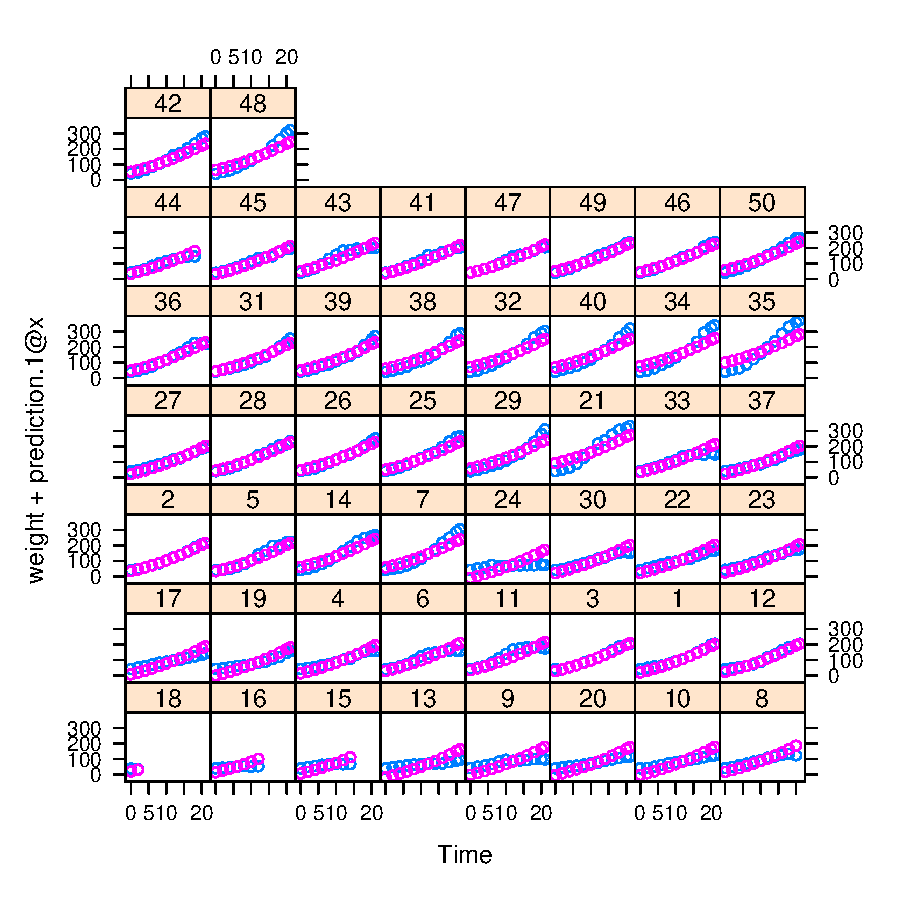
\includegraphics{Lecture4-014}
\end{center}
\caption{Weights of each chick as a function of age in blue, with the predicted weights in purple. A quadratic population growth curve was fitted with random chick intercepts.}
\label{CWpred.1-fig}
\end{figure}

The predictions don't look that bad, but you will notice that for some chicks (e.g. 13,19,34) the slope of the predicted growth seems either to shallow, or too steep. To account for this we can start by fitting \texttt{us(1+time):Chick}. The linear model inside the variance function has two parameters, an intercept (\texttt{1}) and a regression slope associated with \texttt{Time} which define the set of interactions:


\begin{displaymath}
\begin{array}{c|rrrrrc}
&{\color{red} \texttt{Chick1}}&{\color{red} \texttt{Chick2}}&{\color{red} \texttt{Chick3}}&\dots\\
\hline\\
{\color{blue} \texttt{(Intercept)}}&{\color{blue} \texttt{(Intercept)}}.{\color{red} \texttt{Chick1}}&{\color{blue} \texttt{(Intercept)}}.{\color{red} \texttt{Chick2}}&{\color{blue} \texttt{(Intercept)}}.{\color{red} \texttt{Chick3}}&\dots\\
{\color{blue} \texttt{Time}}&{\color{blue} \texttt{Time}}.{\color{red} \texttt{Chick1}}&{\color{blue} \texttt{Time}}.{\color{red} \texttt{Chick2}}&{\color{blue} \texttt{Time}}.{\color{red} \texttt{Chick3}}&\dots\\
\end{array}
\end{displaymath}

Each chick now has an intercept and a slope, and because we have used the \texttt{us} function we are estimating the $2\times2$ matrix:

\begin{displaymath}
{\bf V}_{{\color{red} \texttt{Chick}}}=
\left[
\begin{array}{cc}
\sigma^{2}_{\color{blue}\texttt{(Intercept)}}&\sigma_{\color{blue}\texttt{(Intercept)}, \texttt{Time}}\\
\sigma_{\color{blue}\texttt{(Intercept)}, \texttt{Time}}&\sigma^{2}_{\color{blue} \texttt{Time}}\\
\end{array}
\right]
\end{displaymath}

$\sigma^{2}_{\color{blue}\texttt{(Intercept)}}$ is the amount of variation in intercepts between chicks, and $\sigma^{2}_{\color{blue}\texttt{Time}}$ is the amount of variation in the regression slopes between chicks. If the \texttt{idh} function had been used the covariance would have been set to zero and we could have interpreted variation in intercepts as variation in overall size, and variation in slopes as variation in growth rate.  However, there is often covariance between intercepts and slopes and it is usually a good idea to use the \texttt{us} function and estimate them (see Section \ref{RRcentering}). We shall do so: 

\begin{Schunk}
\begin{Sinput}
> prior.m4a.2 <- list(R = list(V = 1e-16, nu = -2), G = list(G1 = list(V = diag(2), 
+     nu = 2)))
> m4a.2 <- MCMCglmm(weight ~ Diet + poly(Time, 2, raw = TRUE), 
+     random = ~us(1 + Time):Chick, data = ChickWeight, verbose = FALSE, 
+     pr = TRUE, prior = prior.m4a.2, saveX = TRUE, saveZ = TRUE)
\end{Sinput}
\end{Schunk}


\begin{figure}[!h]
\begin{center}
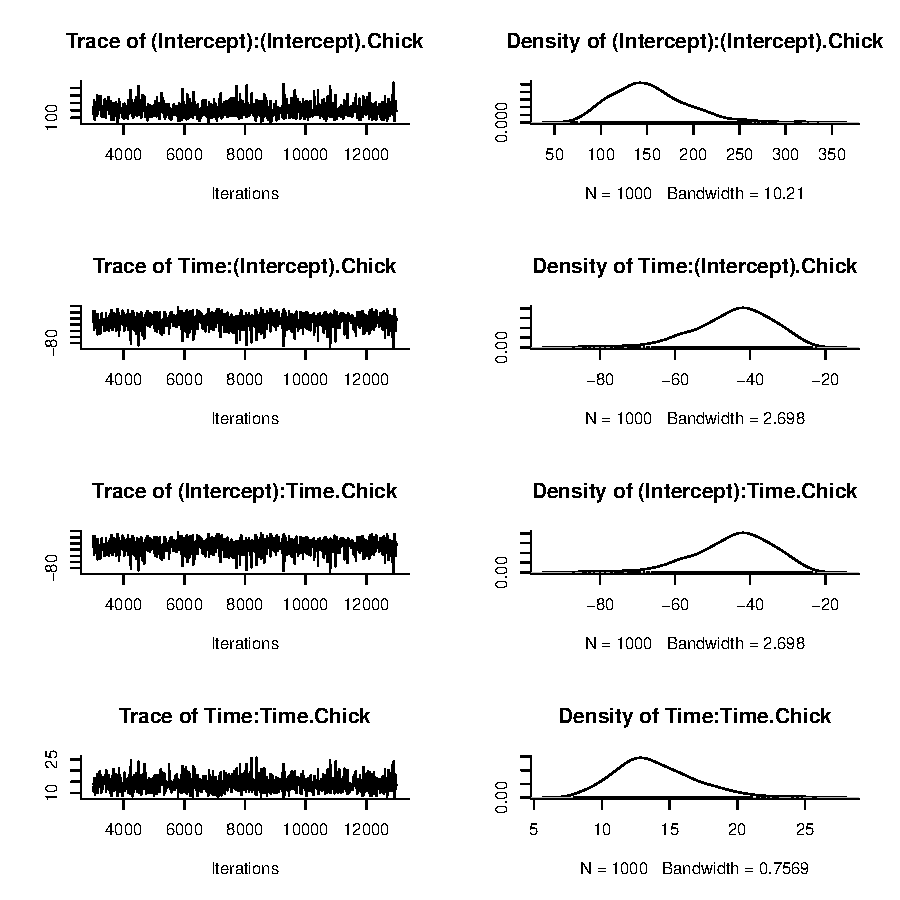
\includegraphics{Lecture4-017}
\end{center}
\caption{MCMC summary plots for the chick covariance components from model \texttt{m4a.2}. The lower and upper plots are the intercept and slope variance components respectively, and the middle two plots are the intercept-slope covariance.}
\label{RR2VCV-fig}
\end{figure}

The traces look OKish for the chick (co)variance matrices (Figure \ref{RR2VCV-fig}) but notice that the the estimate of intercept-slope correlation is close to the boundary of parameter space (-1):

\begin{Schunk}
\begin{Sinput}
> int.slope.cor <- m4a.2$VCV[, 2]/sqrt(m4a.2$VCV[, 1] * m4a.2$VCV[, 
+     4])
> posterior.mode(int.slope.cor)
\end{Sinput}
\begin{Soutput}
      var1 
-0.9767131 
\end{Soutput}
\end{Schunk}

and shows strong autocorrelation

\begin{Schunk}
\begin{Sinput}
> autocorr(int.slope.cor)
\end{Sinput}
\begin{Soutput}
, , 1

                [,1]
Lag 0    1.000000000
Lag 10   0.213576035
Lag 50   0.002312814
Lag 100 -0.020849608
Lag 500 -0.095313496
\end{Soutput}
\end{Schunk}

and we should run it for longer in order to sample the posterior adequately. For now we will carry on and obtain the predictions from the model we ran, but using the \texttt{perdict} function rather than dong it `by hand': 

\begin{Schunk}
\begin{Sinput}
> xyplot(weight + predict(m4a.2, marginal = NULL) ~ Time | Chick, 
+     data = ChickWeight)
\end{Sinput}
\end{Schunk}


\begin{figure}[!h]
\begin{center}
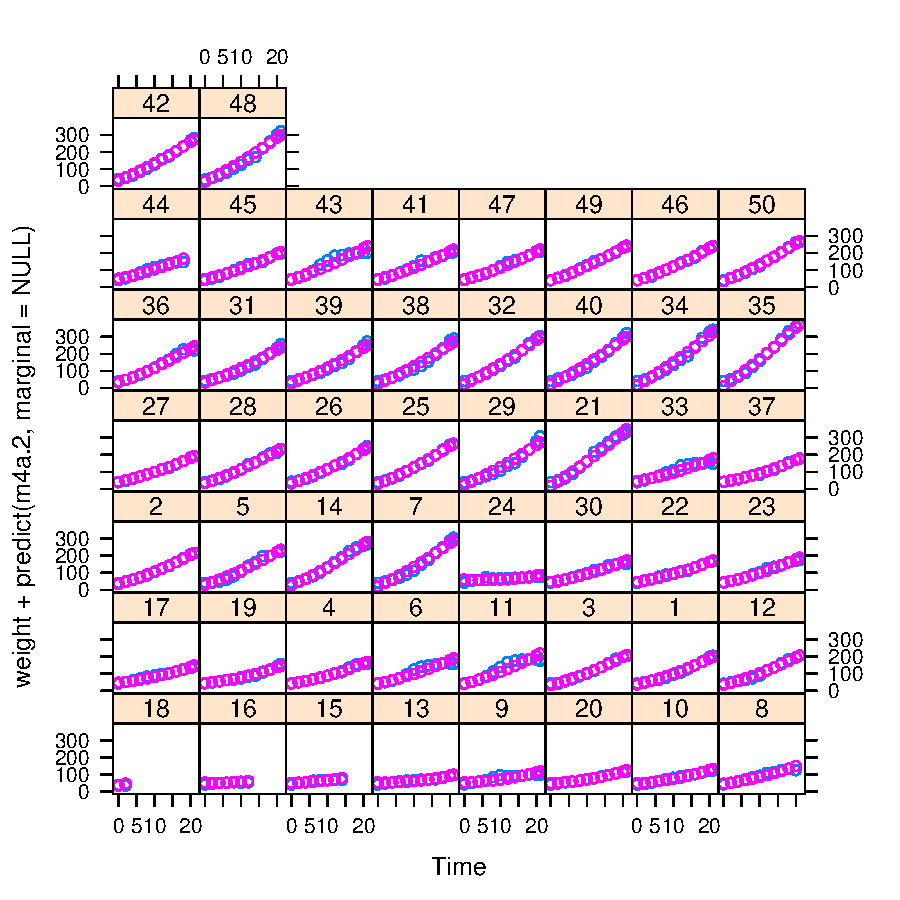
\includegraphics{Lecture4-022}
\end{center}
\caption{Weights of each chick as a function of age in blue, with the predicted weights in purple. A quadratic population growth curve was fitted with a first order random regression for chicks (i.e. a random intercept-slope model).}
\label{CWpred.2-fig}
\end{figure}

and we can see that the fit is much better (See Figure \ref{CWpred.2-fig}). In theory we could fit higher order random regressions (data and prior permitting) and use something like DIC to choose which is the best compromise between the fit of the model to the data and how many effective parameters were fitted. For example we could go from the $1^{st}$ order random regression to a $2^{nd}$ order model: 

\begin{Schunk}
\begin{Sinput}
> prior.m4a.3 <- list(R = list(V = 1, n = 0.002), G = list(G1 = list(V = diag(3), 
+     n = 3)))
> m4a.3 <- MCMCglmm(weight ~ Diet + poly(Time, 2, raw = TRUE), 
+     random = ~us(1 + poly(Time, 2, raw = TRUE)):Chick, data = ChickWeight, 
+     verbose = FALSE, pr = TRUE, prior = prior.m4a.3, saveX = TRUE, 
+     saveZ = TRUE)
\end{Sinput}
\end{Schunk}

and obtain the $3\times3$ covariance matrix:

\begin{displaymath}
{\bf V}_{{\color{red} \texttt{Chick}}}=
\left[
\begin{array}{ccc}
\sigma^{2}_{\color{blue}\texttt{(Intercept)}}&\sigma_{\color{blue}\texttt{(Intercept)}, \texttt{Time}}&\sigma_{\color{blue}\texttt{(Intercept)}, \texttt{Time$^{2}$}}\\
\sigma_{\color{blue}\texttt{(Intercept)}, \texttt{Time}}&\sigma^{2}_{\color{blue} \texttt{Time}}&\sigma_{\color{blue}\texttt{Time}, \texttt{Time$^{2}$}}\\
\sigma_{\color{blue}\texttt{(Intercept)}, \texttt{Time$^2$}}&\sigma_{\color{blue}\texttt{Time}, \texttt{Time$^{2}$}}&\sigma^{2}_{\color{blue} \texttt{Time$^2$}}\\
\end{array}
\right]
\end{displaymath}

The model predicts the chick weights to an even better degree  (See Figure \ref{CWpred.3-fig})

\begin{Schunk}
\begin{Sinput}
> xyplot(weight + predict(m4a.3, marginal = NULL) ~ Time | Chick, 
+     data = ChickWeight)
\end{Sinput}
\end{Schunk}


\begin{figure}[!h]
\begin{center}
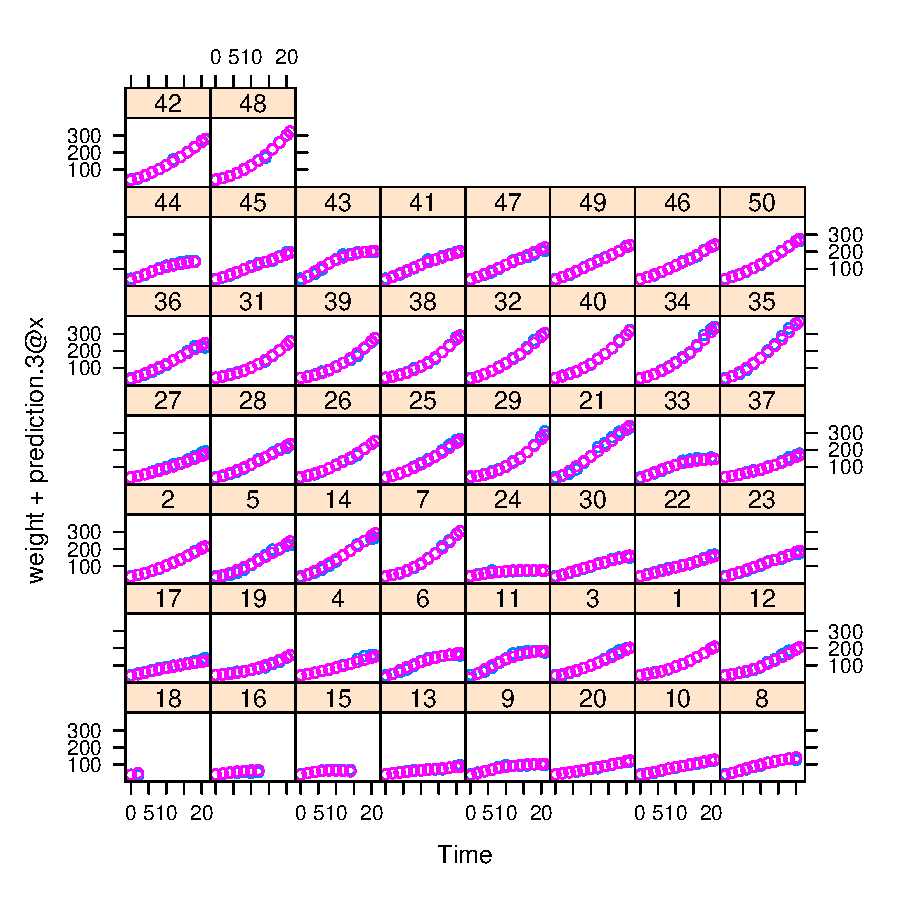
\includegraphics{Lecture4-026}
\end{center}
\caption{Weights of each chick as a function of age in blue, with the predicted weights in purple. A quadratic population growth curve was fitted with a second order random regression for chicks (i.e. a random intercept-slope-quadratic model).}
\label{CWpred.3-fig}
\end{figure}

and the DIC has gone down, suggesting that the model is better:

\begin{Schunk}
\begin{Sinput}
> m4a.1$DIC
\end{Sinput}
\begin{Soutput}
[1] 5525.669
\end{Soutput}
\begin{Sinput}
> m4a.2$DIC
\end{Sinput}
\begin{Soutput}
[1] 4544.62
\end{Soutput}
\begin{Sinput}
> m4a.3$DIC
\end{Sinput}
\begin{Soutput}
[1] 3932.942
\end{Soutput}
\end{Schunk}

It is worth seeing whether using an AIC measure using REML also suggests the highest order model is the better model. 

\begin{Schunk}
\begin{Sinput}
> library(lme4, warn.conflicts = FALSE)
> m5a.1.REML <- lmer(weight ~ Diet + poly(Time, 2, raw = TRUE) + 
+     (1 | Chick), data = ChickWeight)
> summary(m5a.1.REML)@AICtab[1]
\end{Sinput}
\begin{Soutput}
      AIC
 5578.963
\end{Soutput}
\begin{Sinput}
> m5a.2.REML <- lmer(weight ~ Diet + poly(Time, 2, raw = TRUE) + 
+     (poly(Time, 1, raw = TRUE) | Chick), data = ChickWeight)
> summary(m5a.2.REML)@AICtab[1]
\end{Sinput}
\begin{Soutput}
      AIC
 4732.387
\end{Soutput}
\begin{Sinput}
> m5a.3.REML <- lmer(weight ~ Diet + poly(Time, 2, raw = TRUE) + 
+     (poly(Time, 2, raw = TRUE) | Chick), data = ChickWeight)
> summary(m5a.3.REML)@AICtab[1]
\end{Sinput}
\begin{Soutput}
      AIC
 4274.606
\end{Soutput}
\begin{Sinput}
> detach(package:lme4)
\end{Sinput}
\end{Schunk}

\section{Expected Variances and Covariances}

Random regression models make strong assumptions about how the variance should change as a function of the predictor variable. Imagine that the intercept variance was zero, such that all regressions give the same prediction when \texttt{Time}=0. Imagine also that there was variance for slope, the predictions would look something like this (Figure \ref{RRtoy-fig}):

\begin{Schunk}
\begin{Sinput}
> slope <- rnorm(30)
> plot(0, type = "n", xlim = c(-1, 1), ylim = c(-3, 3), ylab = "y", 
+     xlab = "Time")
> for (i in 1:30) {
+     lines(c(-1, 1), c(-slope[i], slope[i]))
+ }
\end{Sinput}
\end{Schunk}

\begin{figure}[!h]
\begin{center}
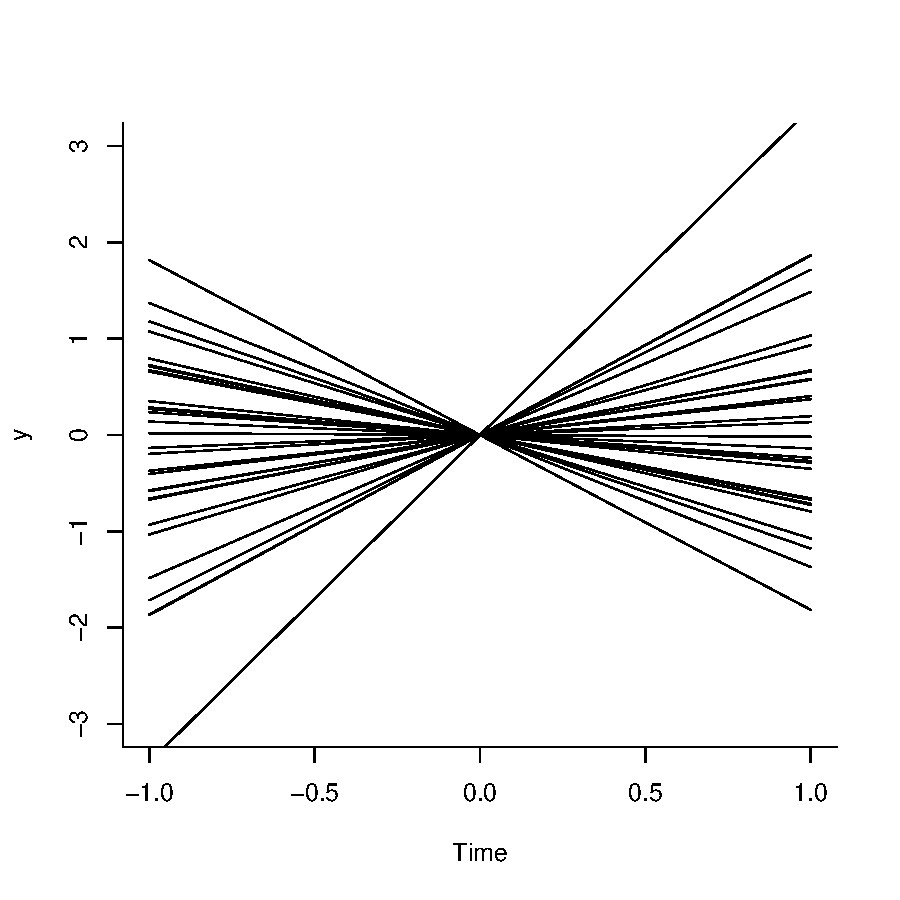
\includegraphics{Lecture4-030}
\end{center}
\caption{Hypothetical regression lines where the variance in slopes is one but the variance in intercepts is zero. The expected variance of y is a quadratic function of Time, being zero when Time=0, and increasing with positive or negative values.}
\label{RRtoy-fig}
\end{figure}


with the variance increasing at extreme values of \texttt{Time} and being zero at \texttt{Time}=0.  For an intercept-slope model such as this the expected variance is quadratic in the predictor, and for a intercept-slope-quadratic model the variance is cubic in the predictor. Generally the expected variance can be obtained using:

\begin{displaymath}
VAR[y] = \textrm{diag}({\bf Z}{\bf V}{\bf Z}^{'})
\label{RRvar-eq}
\end{displaymath}
  
and we can use this to predict the change in variance as a function of \texttt{Time} for the three models:


\begin{Schunk}
\begin{Sinput}
> pos.time <- seq(0, 21, length = 100)
> polynomial <- leg(pos.time, 2, normalized = FALSE)
> beta.1 <- c(posterior.mode(m4a.1$Sol[, 1]), posterior.mode(m4a.1$Sol[, 
+     5]), posterior.mode(m4a.1$Sol[, 6]))
> beta.2 <- c(posterior.mode(m4a.2$Sol[, 1]), posterior.mode(m4a.2$Sol[, 
+     5]), posterior.mode(m4a.2$Sol[, 6]))
> beta.3 <- c(posterior.mode(m4a.3$Sol[, 1]), posterior.mode(m4a.3$Sol[, 
+     5]), posterior.mode(m4a.3$Sol[, 6]))
> VCV.1 <- matrix(posterior.mode(m4a.1$VCV)[1], 1, 1)
> VCV.2 <- matrix(posterior.mode(m4a.2$VCV)[1:(2^2)], 2, 2)
> VCV.3 <- matrix(posterior.mode(m4a.3$VCV)[1:(3^2)], 3, 3)
> units.1 <- posterior.mode(m4a.1$VCV)[2]
> units.2 <- posterior.mode(m4a.2$VCV)[5]
> units.3 <- posterior.mode(m4a.3$VCV)[10]
\end{Sinput}
\end{Schunk}

\iftalk
\begin{Schunk}
\begin{Sinput}
> plot(weight ~ Time, data = ChickWeight, cex.lab = 1.5)
> mu.1 <- polynomial %*% beta.1
> sd.1 <- sqrt(units.1 + diag(polynomial[, 1, drop = FALSE] %*% 
+     VCV.1 %*% t(polynomial[, 1, drop = FALSE])))
> lines(mu.1 ~ pos.time, lwd = 2)
> lines(I(mu.1 + 1.96 * sd.1) ~ pos.time, lty = 2, lwd = 2)
> lines(I(mu.1 - 1.96 * sd.1) ~ pos.time, lty = 2, lwd = 2)
\end{Sinput}
\end{Schunk}
\else
\begin{Schunk}
\begin{Sinput}
> plot(weight ~ Time, data = ChickWeight)
> mu.1 <- polynomial %*% beta.1
> sd.1 <- sqrt(units.1 + diag(polynomial[, 1, drop = FALSE] %*% 
+     VCV.1 %*% t(polynomial[, 1, drop = FALSE])))
> lines(mu.1 ~ pos.time)
> lines(I(mu.1 + 1.96 * sd.1) ~ pos.time, lty = 2)
> lines(I(mu.1 - 1.96 * sd.1) ~ pos.time, lty = 2)
\end{Sinput}
\end{Schunk}
\fi

\begin{figure}[!h]
\begin{center}
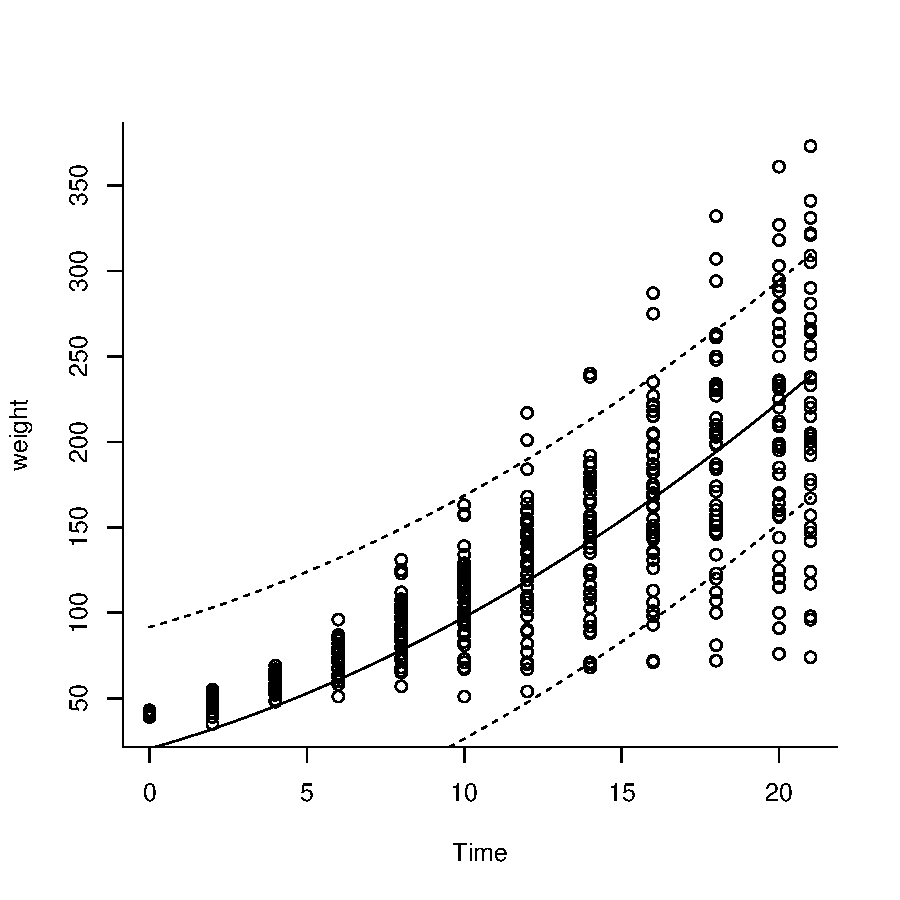
\includegraphics{Lecture4-034}
\end{center}
\caption{Chick weights plotted as a function of time. 95\% of the data are expected to fall within the dashed lines assuming the model with random intercepts is the correct model, and the diet treatments have small effects.}
\label{VCVpred.1-fig}
\end{figure}

The simple model, without a slope term has constant variance across the range, and is clearly inconsistent with the data (Figure \ref{VCVpred.1-fig}). The second model on the other hand

\iftalk
\begin{Schunk}
\begin{Sinput}
> plot(weight ~ Time, data = ChickWeight, cex.lab = 1.5)
> mu.2 <- polynomial %*% beta.2
> sd.2 <- sqrt(units.2 + diag(polynomial[, 1:2, drop = FALSE] %*% 
+     VCV.2 %*% t(polynomial[, 1:2, drop = FALSE])))
> lines(mu.2 ~ pos.time, lwd = 2)
> lines(I(mu.2 + 1.96 * sd.2) ~ pos.time, lty = 2, lwd = 2)
> lines(I(mu.2 - 1.96 * sd.2) ~ pos.time, lty = 2, lwd = 2)
\end{Sinput}
\end{Schunk}
\else
\begin{Schunk}
\begin{Sinput}
> plot(weight ~ Time, data = ChickWeight)
> mu.2 <- polynomial %*% beta.2
> sd.2 <- sqrt(units.2 + diag(polynomial[, 1:2, drop = FALSE] %*% 
+     VCV.2 %*% t(polynomial[, 1:2, drop = FALSE])))
> lines(mu.2 ~ pos.time)
> lines(I(mu.2 + 1.96 * sd.2) ~ pos.time, lty = 2)
> lines(I(mu.2 - 1.96 * sd.2) ~ pos.time, lty = 2)
\end{Sinput}
\end{Schunk}
\fi

\begin{figure}[!h]
\begin{center}
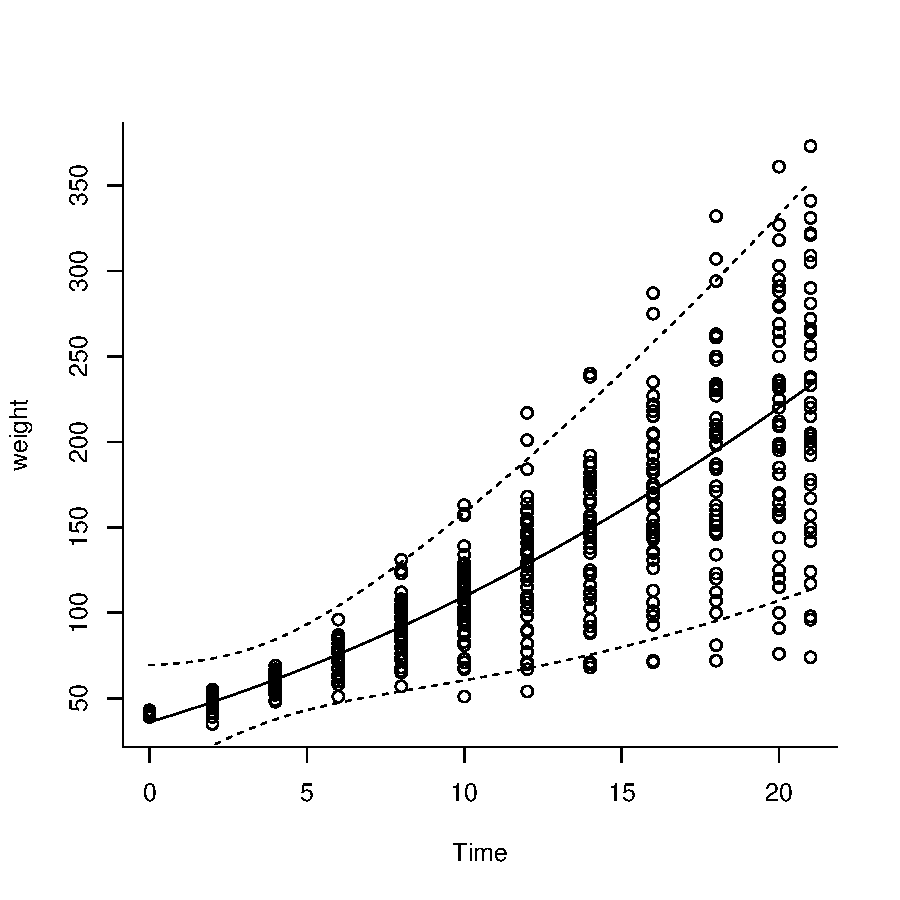
\includegraphics{Lecture4-037}
\end{center}
\caption{Chick weights plotted as a function of time. 95\% of the data are expected to fall within the dashed lines assuming the model with random intercepts and slopes is the correct model, and the diet treatments have small effects.}
\label{VCVpred.2-fig}
\end{figure}

has an expected variance structure reasonably close to that observed (Figure \ref{VCVpred.2-fig}). The highest order model, which was the best using information criteria such as AIC an DIC, also does badly (Figure \ref{VCVpred.3-fig}): 

\iftalk
\begin{Schunk}
\begin{Sinput}
> plot(weight ~ Time, data = ChickWeight, ylim = c(-150, 600), 
+     cex.lab = 1.5)
> mu.3 <- polynomial %*% beta.3
> sd.3 <- sqrt(units.3 + diag(polynomial[, 1:3, drop = FALSE] %*% 
+     VCV.3 %*% t(polynomial[, 1:3, drop = FALSE])))
> lines(mu.3 ~ pos.time, lwd = 2)
> lines(I(mu.3 + 1.96 * sd.3) ~ pos.time, lty = 2, lwd = 2)
> lines(I(mu.3 - 1.96 * sd.3) ~ pos.time, lty = 2, lwd = 2)
\end{Sinput}
\end{Schunk}
\else
\begin{Schunk}
\begin{Sinput}
> plot(weight ~ Time, data = ChickWeight, ylim = c(-150, 600))
> mu.3 <- polynomial %*% beta.3
> sd.3 <- sqrt(units.3 + diag(polynomial[, 1:3, drop = FALSE] %*% 
+     VCV.3 %*% t(polynomial[, 1:3, drop = FALSE])))
> lines(mu.3 ~ pos.time)
> lines(I(mu.3 + 1.96 * sd.3) ~ pos.time, lty = 2)
> lines(I(mu.3 - 1.96 * sd.3) ~ pos.time, lty = 2)
\end{Sinput}
\end{Schunk}
\fi

\begin{figure}[!h]
\begin{center}
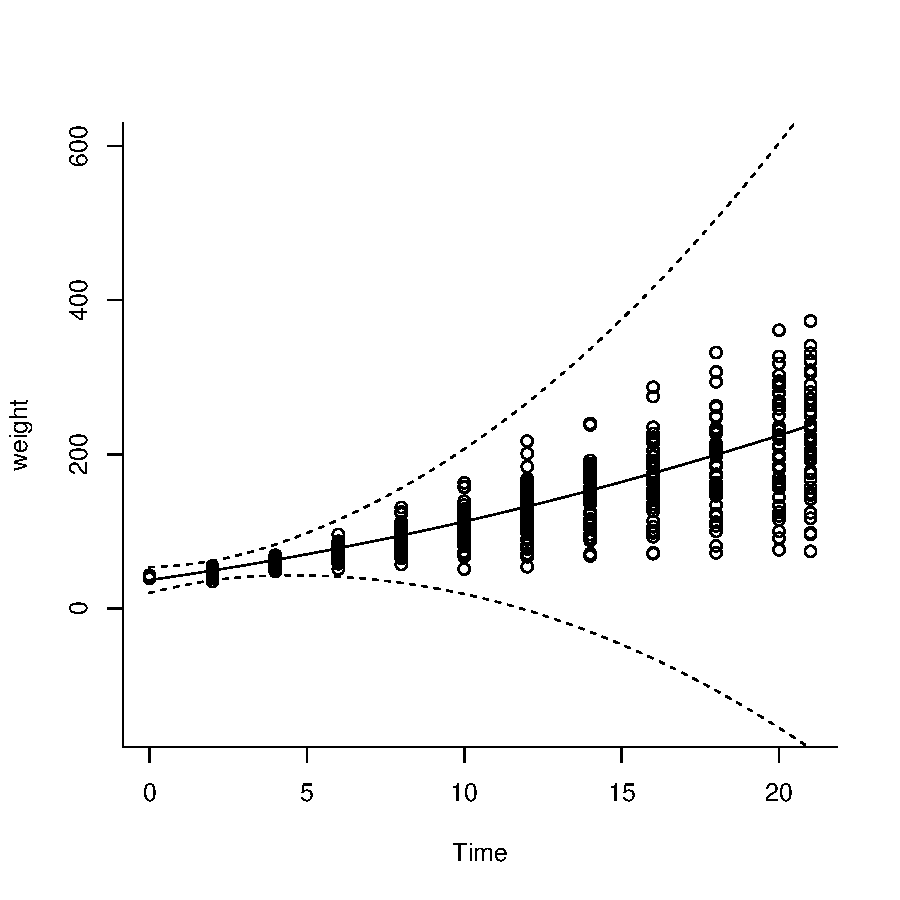
\includegraphics{Lecture4-040}
\end{center}
\caption{Chick weights plotted as a function of time. 95\% of the data are expected to fall within the dashed lines assuming the model with random intercepts, slopes and quadratic effects is the correct model, and the diet treatments have small effects.}
\label{VCVpred.3-fig}
\end{figure}

In general, I would not draw conclusions about changes in variance from random regression models \citep{Pletcher.1999a}.

\section{\texttt{us} versus \texttt{idh} and mean centering}
\label{RRcentering}
bad\\ 
reparametersitaion\\

\begin{Schunk}
\begin{Sinput}
> prior.m4b.1 <- list(R = list(V = 1e-16, nu = -2), G = list(G1 = list(V = diag(2), 
+     nu = 2)))
> m4b.1 <- MCMCglmm(weight ~ Diet + poly(Time, 2, raw = TRUE), 
+     random = ~us(1 + I(Time - 3)):Chick, data = ChickWeight, 
+     verbose = FALSE, pr = TRUE, prior = prior.m4b.1, saveX = TRUE, 
+     saveZ = TRUE)
\end{Sinput}
\end{Schunk}

\section{Meta-analysis}
\label{meta-sec}

Random intercept-slope models implicitly assume that the variance changes as a quadratic function of the predictor. This can be used to our advantage because it allows us to fit meta-analytic models. In meta-analysis the data are usually some standardised statistic which has been estimated with different levels of measurement error. If we wanted to know the expected value of these statistics we would want to weight our answer to those measurements made with the smallest amount of error.  If we assume that measurement error around the true value is normally distributed then we could assume the model:


\begin{equation}
y_{i} = \beta_{1} + m_{i} +e _{i}
\end{equation} 
 
where $\beta_{1}$ is the expected value, $m_{i}$ is some deviation due to measurement error, and $e_{i}$ is the deviation of the statistic from the global intercept not due to measurement error. Some types of meta-analysis presume $e_{i}$ does not exist and that the only variation between studies is due to measurement error. This is not realistic, I think.  Often, standard errors are reported in the literature, and these can be viewed as an approximation to the expected standard deviation of the measurement error. If we put the standard errors for each statistic as a column in the data frame (and call it \texttt{SE}) then the random term \texttt{idh(SE):units} defines a diagonal matrix with the standard errors on the diagonal. Using results from Equation \ref{RRvar-eq}


\begin{equation}
\begin{array}{rl}
\textrm{VAR}[{\bf m}] =& {\bf Z}{\bf V}{\bf Z}^{'}\\ 
               =& {\bf Z}\sigma^{2}_{m}{\bf I}{\bf Z}^{'}\\ 
               =& \sigma^{2}_{m}{\bf Z}{\bf Z}^{'}\\                               
\end{array}
\end{equation} 

fixing $\sigma^{2}_{m}=1$ in the prior, the expected variance in the measurement errors are therefore the standard errors squared (the sampling variance) and all measurement errors are assumed to be independent of each other. The random regression therefore fits a random effect meta-analysis.   

\section{Splines}

blah blah

\begin{Schunk}
\begin{Sinput}
> random = ~idv(spl(covariate))
\end{Sinput}
\end{Schunk}

fits a penalised thin-plate spline,

\begin{Schunk}
\begin{Sinput}
> random = ~idv(smspline(covariate))
\end{Sinput}
\end{Schunk}

fits a penalised cubic spline. The coefficients are random effects, stored in the \texttt{Sol} element of the model output and the single variance component (the penalising bit) is in the \texttt{VCV} element. Its usually a good idea to scale the covariate to lie in the interval [0,1] or some such thing. 


\ifalone
\end{document}
\else
\fi

